\chapter{Generalization}

\vspace{1em}
\hfill
\begin{minipage}[c]{0.55\textwidth}
\raggedleft
\small\itshape
In the absence of any specific knowledge about the problem, no algorithm can be expected to outperform any other.\\[0.5em]
\upshape\footnotesize David H. Wolpert and William G. Macready, ``No Free Lunch Theorems for Optimization'' (1997)
\end{minipage}%
\hspace{0.5em}
\begin{minipage}[c]{0.12\textwidth}
% \includegraphics[width=\textwidth]{figures/ch07_generalization.png}
\end{minipage}
\vspace{1.5em}

\noindent The previous chapter ended with a problem. Tabular Q-learning works on toy environments but does not scale. Chess has about $10^{44}$ legal positions. Go has about $10^{170}$. Even Pac-Man has more states than an agent can visit in any feasible amount of training. Almost every state the agent encounters in play is new: it has never seen exactly this configuration before.

A tabular agent has nothing to say about a state it has not seen. Its $Q$-table has no entry. It cannot \emph{generalize}.

Generalization is the central problem of machine learning. Given a finite sample of experience, the agent has to behave sensibly on the much larger universe of situations it has not yet seen. This chapter is about how that works, why it is possible at all, and what it costs.

\section*{From a table to a function}

The fix is to stop thinking about $Q$ as a table and start thinking about it as a function. The Q-value $Q(s, a)$ becomes the output of a parameterized function $Q_\theta(s, a)$, where $\theta$ are the function's parameters. Figure~\ref{fig:tabular-vs-parametric} shows the difference.

\begin{figure}[h]
\centering
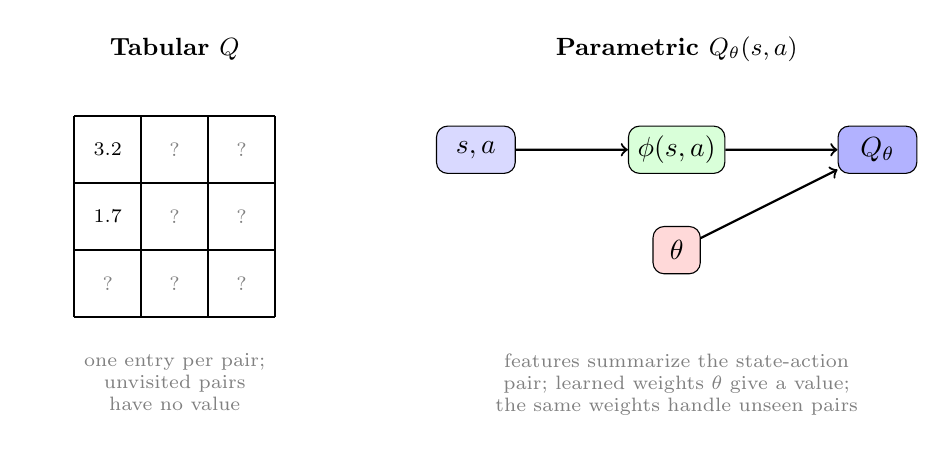
\begin{tikzpicture}[scale=0.85]
  % Left: tabular
  \node[font=\small\bfseries] at (1.5, 4) {Tabular $Q$};
  \draw[thick] (0, 0) grid (3, 3);
  \node[font=\scriptsize] at (0.5, 2.5) {3.2};
  \node[font=\scriptsize, gray] at (1.5, 2.5) {?};
  \node[font=\scriptsize, gray] at (2.5, 2.5) {?};
  \node[font=\scriptsize] at (0.5, 1.5) {1.7};
  \node[font=\scriptsize, gray] at (1.5, 1.5) {?};
  \node[font=\scriptsize, gray] at (2.5, 1.5) {?};
  \node[font=\scriptsize, gray] at (0.5, 0.5) {?};
  \node[font=\scriptsize, gray] at (1.5, 0.5) {?};
  \node[font=\scriptsize, gray] at (2.5, 0.5) {?};
  \node[font=\scriptsize, anchor=north, text width=3.5cm, align=center, gray] at (1.5, -0.4) {one entry per pair;\\unvisited pairs have no value};

  % Right: parametric
  \node[font=\small\bfseries] at (9, 4) {Parametric $Q_\theta(s, a)$};
  \node[draw, fill=blue!15, rounded corners, minimum width=1cm, minimum height=0.6cm] (state) at (6, 2.5) {$s, a$};
  \node[draw, fill=green!15, rounded corners, minimum width=1.2cm, minimum height=0.6cm] (phi) at (9, 2.5) {$\phi(s, a)$};
  \node[draw, fill=red!15, rounded corners, minimum width=0.6cm, minimum height=0.6cm] (theta) at (9, 1) {$\theta$};
  \node[draw, fill=blue!30, rounded corners, minimum width=1cm, minimum height=0.6cm] (q) at (12, 2.5) {$Q_\theta$};
  \draw[->, thick] (state) -- (phi);
  \draw[->, thick] (phi) -- (q);
  \draw[->, thick] (theta) -- (q);
  \node[font=\scriptsize, anchor=north, text width=5cm, align=center, gray] at (9, -0.4) {features summarize the state-action pair; learned weights $\theta$ give a value; the same weights handle unseen pairs};
\end{tikzpicture}
\caption{Tabular vs parametric Q. The tabular Q-function stores one estimate per state-action pair; unseen pairs have no value. The parametric Q-function processes any state-action pair through features and a shared set of learned weights, producing values even for pairs the agent has never seen. Generalization comes from the function's structure, not from individual observations.}
\label{fig:tabular-vs-parametric}
\end{figure}

The agent learns $\theta$ from experience. When it observes $(s, a, r, s')$, instead of updating one table entry, it updates $\theta$ in the direction that makes $Q_\theta(s, a)$ closer to the temporal-difference target. The update typically changes $Q_\theta$ at \emph{other} state-action pairs too, including pairs the agent has never visited. The function generalizes.

The simplest case is linear function approximation. Define a feature vector $\phi(s, a)$ describing the state-action pair. Approximate $Q(s, a) \approx \theta^T \phi(s, a)$. Learn $\theta$ by gradient descent.

For Pac-Man, useful features might be: distance to the nearest ghost, distance to the nearest food pellet, how many ghosts are in scared mode, whether a power pellet is reachable. A handful of carefully chosen features with learned weights can produce a competent Pac-Man player after a few hundred games. A tabular method would need millions.

\section*{Neural networks, briefly}

For most interesting problems, the right features are not obvious. You do not know which projections of the state matter. Then the features themselves have to be learned.

A neural network is a parameterized function $f_\theta: \mathbb{R}^n \to \mathbb{R}^m$. It takes a real-valued input vector and produces a real-valued output vector. The parameters $\theta$ are the weights and biases of its layers. Different choices of $\theta$ give different functions; learning is finding the $\theta$ that fits the training data well.

The simplest version is a single linear layer:

$$\mathbf{z} = W \mathbf{x} + \mathbf{b}.$$

Take an input vector $\mathbf{x}$, multiply by a matrix of weights $W$, add a bias vector $\mathbf{b}$. This is a linear function. It can fit any input-output mapping that is itself linear. It cannot fit anything else. The classic counterexample is the XOR function: it cannot be expressed as a linear combination of its inputs. A single linear unit cannot learn XOR no matter how long you train it.

The fix is to stack layers and put a nonlinear function between them.

$$\mathbf{h}_1 = \sigma(W_1 \mathbf{x} + \mathbf{b}_1)$$
$$\mathbf{h}_2 = \sigma(W_2 \mathbf{h}_1 + \mathbf{b}_2)$$
$$\vdots$$
$$\mathbf{y} = W_L \mathbf{h}_{L-1} + \mathbf{b}_L$$

Here $\sigma$ is a nonlinear function applied componentwise (a common choice is the rectified linear unit, $\sigma(z) = \max(0, z)$). Without $\sigma$, the composition of linear layers is just another linear function. With $\sigma$, the composition can represent functions arbitrarily complex. This is a \emph{multi-layer perceptron} (MLP) or, more loosely, a \emph{deep network} when $L$ is large. Figure~\ref{fig:mlp} shows the structure.

\begin{figure}[h]
\centering
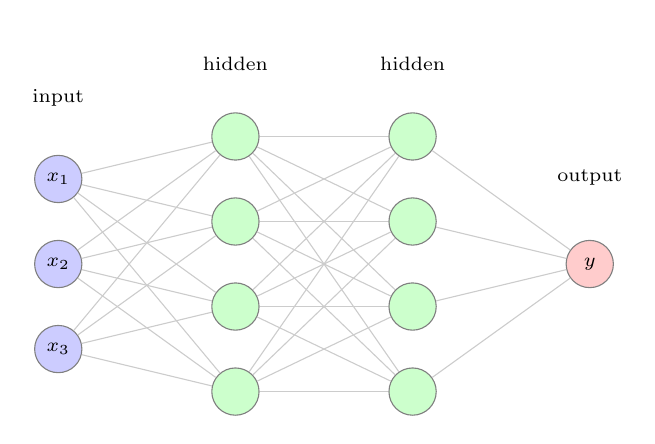
\begin{tikzpicture}[
  scale=0.9,
  every node/.style={circle, draw=gray, minimum size=6mm, font=\scriptsize, inner sep=1pt},
  >=stealth
]
  % Input layer
  \node[fill=blue!20] (x1) at (0, 2.4) {$x_1$};
  \node[fill=blue!20] (x2) at (0, 1.2) {$x_2$};
  \node[fill=blue!20] (x3) at (0, 0) {$x_3$};

  % Hidden 1
  \node[fill=green!20] (h11) at (2.5, 3) {};
  \node[fill=green!20] (h12) at (2.5, 1.8) {};
  \node[fill=green!20] (h13) at (2.5, 0.6) {};
  \node[fill=green!20] (h14) at (2.5, -0.6) {};

  % Hidden 2
  \node[fill=green!20] (h21) at (5, 3) {};
  \node[fill=green!20] (h22) at (5, 1.8) {};
  \node[fill=green!20] (h23) at (5, 0.6) {};
  \node[fill=green!20] (h24) at (5, -0.6) {};

  % Output
  \node[fill=red!20] (y) at (7.5, 1.2) {$y$};

  % Connections (sparse, illustrative)
  \foreach \i in {x1, x2, x3}
    \foreach \j in {h11, h12, h13, h14}
      \draw[gray!40, thin] (\i) -- (\j);
  \foreach \i in {h11, h12, h13, h14}
    \foreach \j in {h21, h22, h23, h24}
      \draw[gray!40, thin] (\i) -- (\j);
  \foreach \i in {h21, h22, h23, h24}
    \draw[gray!40, thin] (\i) -- (y);

  % Labels
  \node[draw=none, font=\scriptsize, anchor=south] at (0, 3.1) {input};
  \node[draw=none, font=\scriptsize, anchor=south] at (2.5, 3.5) {hidden};
  \node[draw=none, font=\scriptsize, anchor=south] at (5, 3.5) {hidden};
  \node[draw=none, font=\scriptsize, anchor=south] at (7.5, 1.9) {output};
\end{tikzpicture}
\caption{A small multi-layer perceptron with three input units, two hidden layers of four units each, and one output. Every edge is a learned weight; every hidden unit applies a nonlinear activation to its weighted sum of inputs. The function as a whole is parameterized by the collection of all weights. Real networks are larger (millions to trillions of parameters) and use specialized architectures, but the basic structure is this.}
\label{fig:mlp}
\end{figure}

That is the core picture. Training is finding weights that make the network's outputs match the targets. The algorithm is gradient descent on a loss function; the gradient is computed efficiently by backpropagation (Rumelhart, Hinton, Williams 1986). The mathematics is not particularly difficult; the engineering challenge has been building hardware and software that can handle networks at the scales modern problems demand.

In the RL setting, the Q-function $Q_\theta(s, a)$ is the output of a neural network. The state goes in (as raw pixels, as encoded features, as a token sequence); the value comes out. Deep Q-Networks (DeepMind 2013) applied this to Atari games, achieving superhuman performance on most of them using only raw pixel input. AlphaGo (2016) combined deep networks with tree search and beat the human world champion at Go. The pattern is the same: the network learns whatever features matter for value.

\section*{Everything is a universal approximator}

A point worth making explicit, because the rest of the chapter hinges on it.

The table from the previous section is a universal function approximator. Given enough rows, it can represent any function from inputs to outputs exactly. A linear model is also universal in the trivial sense of representing every linear function. A multi-layer perceptron is universal in a deeper sense: Cybenko (1989) and Hornik (1991) proved that an MLP with one hidden layer and enough units can approximate any continuous function on a bounded domain to arbitrary precision. Convolutional networks, recurrent networks, transformers, mixtures of experts: all universal in the same approximation-theoretic sense.

Universality is cheap. Approximating any function in the limit, given unlimited capacity and unlimited data, is not the interesting property. The interesting property is sample efficiency: how much data does the representation need before it generalizes correctly to inputs it has not seen?

A table needs one observation per cell. A linear model with $k$ features needs on the order of $k$ observations to fit. A transformer trained on internet-scale text can sometimes generalize from a handful of in-context examples to tasks it was never explicitly trained on, because its architecture imposes structure that lets it interpolate across nearby inputs without having seen them.

This is the load-bearing fact: the choice of representation is not a choice about what the system can in principle compute. It is a choice about what kinds of inputs it can generalize across efficiently. The representation is where the inductive bias lives.

A useful way to see this is to think of the representation as a geometry over the input space. The architecture is a recipe for mapping inputs to points in some feature space. If similar inputs (in the sense that matters for the task) land in nearby points, the network's learned function will produce sensible outputs on unseen nearby inputs by continuity. If similar inputs land in unrelated points, the network has to learn each one separately, and finite data will not be enough. The art of architecture design is arranging the geometry so that the similarities that matter become spatial closeness in the representation. Figure~\ref{fig:representation-geometry} shows the difference.

\begin{figure}[h]
\centering
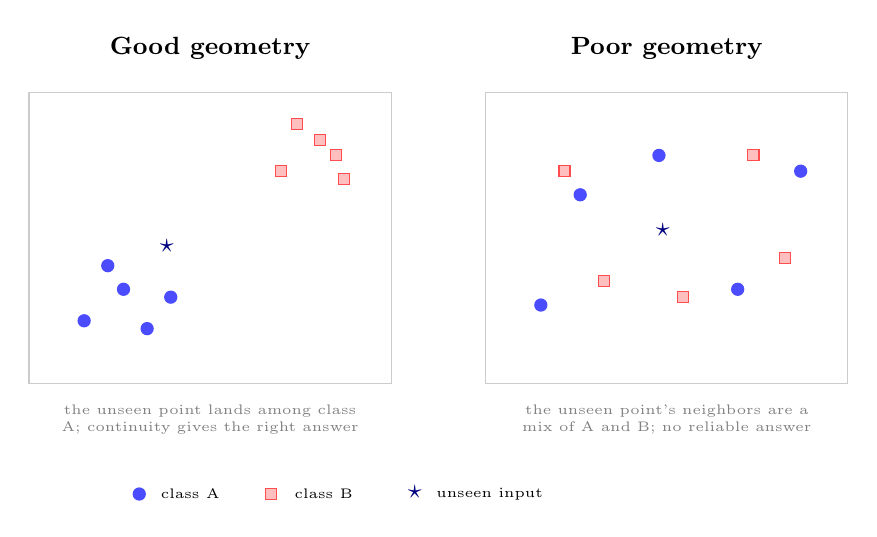
\begin{tikzpicture}[scale=1.0]
  % ---- Left panel: good geometry ----
  \node[font=\small\bfseries, anchor=south] at (2.3, 4.0) {Good geometry};
  \draw[gray!40] (0,0) rectangle (4.6,3.7);
  \foreach \x/\y in {0.7/0.8, 1.2/1.2, 1.5/0.7, 1.0/1.5, 1.8/1.1} {\fill[blue!70] (\x,\y) circle (2.4pt);}
  \foreach \x/\y in {3.2/2.7, 3.7/3.1, 4.0/2.6, 3.4/3.3, 3.9/2.9} {\draw[red!70, fill=red!25] (\x-0.07,\y-0.07) rectangle (\x+0.07,\y+0.07);}
  \node[blue!50!black] at (1.75, 1.75) {$\star$};
  \node[font=\tiny, gray, anchor=north, text width=4.4cm, align=center] at (2.3, -0.15) {the unseen point lands among class A; continuity gives the right answer};

  % ---- Right panel: poor geometry ----
  \node[font=\small\bfseries, anchor=south] at (8.1, 4.0) {Poor geometry};
  \draw[gray!40] (5.8,0) rectangle (10.4,3.7);
  \foreach \x/\y in {6.5/1.0, 8.0/2.9, 9.0/1.2, 7.0/2.4, 9.8/2.7} {\fill[blue!70] (\x,\y) circle (2.4pt);}
  \foreach \x/\y in {6.8/2.7, 8.3/1.1, 9.2/2.9, 7.3/1.3, 9.6/1.6} {\draw[red!70, fill=red!25] (\x-0.07,\y-0.07) rectangle (\x+0.07,\y+0.07);}
  \node[blue!50!black] at (8.05, 1.95) {$\star$};
  \node[font=\tiny, gray, anchor=north, text width=4.4cm, align=center] at (8.1, -0.15) {the unseen point's neighbors are a mix of A and B; no reliable answer};

  % ---- Legend ----
  \fill[blue!70] (1.4,-1.4) circle (2.4pt);
  \node[font=\tiny, anchor=west] at (1.55,-1.4) {class A};
  \draw[red!70, fill=red!25] (3.0,-1.47) rectangle (3.14,-1.33);
  \node[font=\tiny, anchor=west] at (3.25,-1.4) {class B};
  \node[blue!50!black] at (4.9,-1.38) {$\star$};
  \node[font=\tiny, anchor=west] at (5.05,-1.4) {unseen input};
\end{tikzpicture}
\caption{Representation as geometry. Both panels show the same five examples of class A (circles), five of class B (squares), and one unseen input (star) to be classified. Left: a representation in which the features that matter place each class in its own region. The unseen input lands among class A, and the learned function gives it class A's answer by continuity, without ever having seen it. Right: a representation in which the same inputs scatter. The unseen input's nearest neighbors are a mix of both classes, so no amount of training data on these points tells the function what to do with it. Same inputs, same classes, different geometry; only the left one generalizes.}
\label{fig:representation-geometry}
\end{figure}

Output heads work on the same principle. A linear classification head says ``the right output is a linear combination of these features.'' A softmax over a vocabulary says ``the right output is one of these discrete options, weighted by feature combinations.'' A mixture-of-experts head says ``different inputs should route through different sub-functions.'' Each is a bias about how the representation should combine into outputs.

The sharpest test of whether a representation's biases match the world is not in-distribution sample efficiency, where the test inputs come from the same distribution as the training data. It is out-of-distribution generalization: does the system behave sensibly on inputs that look different from training but share underlying structure? A representation that does well in-distribution and poorly out-of-distribution has learned the surface statistics of the training data without the underlying structure. A representation that does well out-of-distribution has built the right kind of structure into its geometry. Most of what we want from advanced AI systems is OOD generalization in this sense: behaving sensibly on situations the training set did not contain.

\section*{No free lunch}

You do not get function approximation for free.

The \emph{no-free-lunch theorems} (Wolpert and Macready 1997) say that no learning algorithm is uniformly best across all possible problems. Averaged over every conceivable input-output mapping you might want to learn, every algorithm performs the same. Any algorithm that does well on the problems we actually care about (structured environments, hierarchical patterns, discoverable regularities) does so because it has assumptions baked in that match the structure of those problems.

These assumptions are called \emph{inductive biases}. Every learning system has them. The choice of features, the network architecture, the activation function, the regularization, the loss function, the training data: all encode inductive biases. They constrain the space of functions the system can express easily, and that constraint is what lets it learn from finite data.

Different architectures encode different biases:

\begin{itemize}
\item \textbf{Convolutional networks} bias toward translation invariance and local structure: a feature in one part of the image is recognized in any other part. Good for images, where the same patterns recur at different locations.
\item \textbf{Recurrent networks} bias toward sequential dependence: each step's output depends on a hidden state carried from previous steps. Decent for time series; surpassed by transformers for language.
\item \textbf{Transformers} bias toward attention-mediated long-range dependencies: any position in a sequence can directly attend to any other position. The winning architecture for language so far, and increasingly for vision too.
\item \textbf{Pre-trained foundation models} bias toward whatever statistical structure was present in the pre-training data. Training a transformer on internet-scale text bakes in implicit knowledge about language, the world, common arguments, and the structure of human communication. This pre-training is itself an inductive bias for downstream tasks.
\end{itemize}

The choice of architecture is not aesthetic. It is a choice about which problems the system can learn efficiently.

Sample efficiency and inductive bias are two ways of describing the same property. A learner with a perfect inductive bias for a problem learns it from one observation (in the limit). A learner with the wrong inductive bias may never learn it. Most real learners sit somewhere in between. Improving them often means improving the bias more than improving the algorithm.

\section*{Solomonoff as the limit case}

The connection back to Part I: Solomonoff's universal prior is the most general inductive bias possible.

Solomonoff weights hypotheses by description length: $M(x) \approx 2^{-K(x)}$. The bias is ``simpler explanations are more probable.'' It works uniformly across every problem with computable structure, which (under the Church-Turing thesis) is every problem there is. It is universal.

But uncomputable. Real learning systems cannot run Solomonoff. They use bounded inductive biases instead. A transformer's bias is far more restrictive than Solomonoff's, but the transformer is something you can actually train on a real dataset in a finite amount of time. The architecture trades coverage for tractability.

This is the central design trade-off in modern machine learning. Pick a bias too narrow, and you cannot represent what you need. Pick it too broad, and you cannot learn from feasible data. The art is in matching the bias to the structure of the world you want the system to handle.

Figure~\ref{fig:bias-tradeoff} sketches the trade-off.

\begin{figure}[h]
\centering
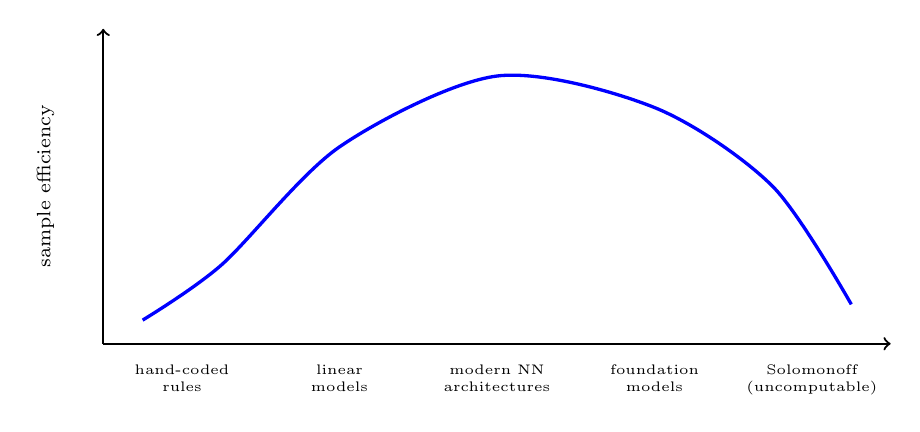
\begin{tikzpicture}[scale=1.0, every node/.style={align=center, font=\scriptsize}]
  % Axes
  \draw[->, thick] (0, 0) -- (10, 0);
  \draw[->, thick] (0, 0) -- (0, 4);
  \node[font=\scriptsize, rotate=90, anchor=south] at (-0.5, 2) {sample efficiency};

  % Curve: peak in middle
  \draw[blue, very thick] plot[smooth, tension=0.5] coordinates {(0.5, 0.3) (1.5, 1.0) (3, 2.5) (5, 3.4) (7, 3.0) (8.5, 2.0) (9.5, 0.5)};

  % Category labels below the x-axis
  \node[anchor=north, font=\tiny, text width=1.6cm] at (1, -0.15) {hand-coded\\rules};
  \node[anchor=north, font=\tiny, text width=1.6cm] at (3, -0.15) {linear\\models};
  \node[anchor=north, font=\tiny, text width=1.8cm] at (5, -0.15) {modern NN\\architectures};
  \node[anchor=north, font=\tiny, text width=1.8cm] at (7, -0.15) {foundation\\models};
  \node[anchor=north, font=\tiny, text width=1.8cm] at (9, -0.15) {Solomonoff\\(uncomputable)};
\end{tikzpicture}
\caption{The inductive-bias trade-off. The horizontal axis is the breadth of inductive bias, from narrow (hand-coded rules) to maximally broad (Solomonoff). The vertical axis is sample efficiency on the kinds of problems the system is actually applied to. A narrow bias cannot express what you need; a maximally broad bias (Solomonoff) covers everything but is uncomputable. The sweet spot for real problems sits somewhere in between: bias broad enough to express the structure of the problem, narrow enough to learn from feasible data. The dominant architectures of modern AI are points on this curve, each a particular bet about which problems matter and what their structure is.}
\label{fig:bias-tradeoff}
\end{figure}

The dominant systems of modern AI (transformers for language, CNNs for vision, RL with deep function approximation for control) are not arbitrary choices. They are particular bets about what inductive biases match the structure of language, of visual scenes, of sequential decision problems. The bets have paid off so far. They have not paid off everywhere; there are domains where current architectures struggle, often because the inductive bias is wrong for the structure of the problem.

\section*{Where this leaves you}

You now have the conceptual machinery for understanding why modern AI looks the way it does. Function approximation replaces the table. Neural networks learn their own features. The choice of architecture is the choice of inductive bias. Sample efficiency comes from biases that match the problem's structure. Solomonoff sits at the limit, universal but unreachable.

This chapter sits at a hinge in the book. Parts I and II built the theory of optimal agency in clean settings (Solomonoff, EU, RL). Part III will treat the specification problem (reward modeling, alignment, oversight) in similarly clean settings. Part IV will move to messy practice: LLMs, what we observe when alignment is tested in real systems, where the gap lives.

But first, one more piece of theory. The next chapter combines the optimal predictor (Part I) and the optimal decider (Chapter 6, plus the generalization machinery of this one) into a single object: AIXI, the optimal universal agent. It is the reference point that the rest of the book points toward, and it is the cleanest statement of what intelligence is in the limit.
